% BEGIN PREAMBEL
\documentclass[9pt]{beamer}
\usepackage[british]{babel}
\usepackage[latin1]{inputenc}
\usepackage{multimedia}
\usepackage{amsmath,amsfonts,amssymb}
\usepackage{upgreek}
\usepackage{pgfpages}
\usepackage[version=3]{mhchem}
\usepackage{lmodern}
\usepackage{graphicx}
\usepackage{multicol}
\usepackage{xcolor}
\usepackage{wrapfig}
\usepackage{siunitx}
\newcommand{\as}{\\[14pt]}
\newcommand{\s}{\\[7pt]}
\newcommand{\is}{\\[2pt]}
\newcommand{\no}{\noindent}
\newcommand{\ka}{\hspace*{0.5cm}}
\newcommand{\ma}{\hspace*{1cm}}
\newcommand{\ga}{\hspace*{1.5cm}}
\newcommand{\li}{\left|}
\newcommand{\re}{\right|}
\newcommand{\const}{\text{const.}}
\newcommand{\z}{\text}
\newcommand{\terminal}[1]{\colorbox{black}{\textcolor{white}{{\fontfamily{phv}\selectfont \scriptsize{#1}}}}}
\newcommand{\plugin}[1]{\textit{\flq#1\frq}}
\usetheme{Boadilla}
\graphicspath{ {Pics/} }
\usecolortheme{beaver}
\useoutertheme{miniframes}
\beamertemplatenavigationsymbolsempty
\makeindex
\title[Analysis]{Rate Pad Analysis}
\author[M. Reichmann]{Michael Reichmann}
\institute[\textbf{\textit{ETH}}\scalebox{.6}{\textit{Z\"{u}rich}}]{Swiss Federal Institute of Technology Zurich}
\AtBeginSection{\frame{\sectionpage}}
% END PREAMBEL
\begin{document}
% ============================
% BEGIN TITLE PAGE
% ============================
\begin{frame}
	\begin{center}
		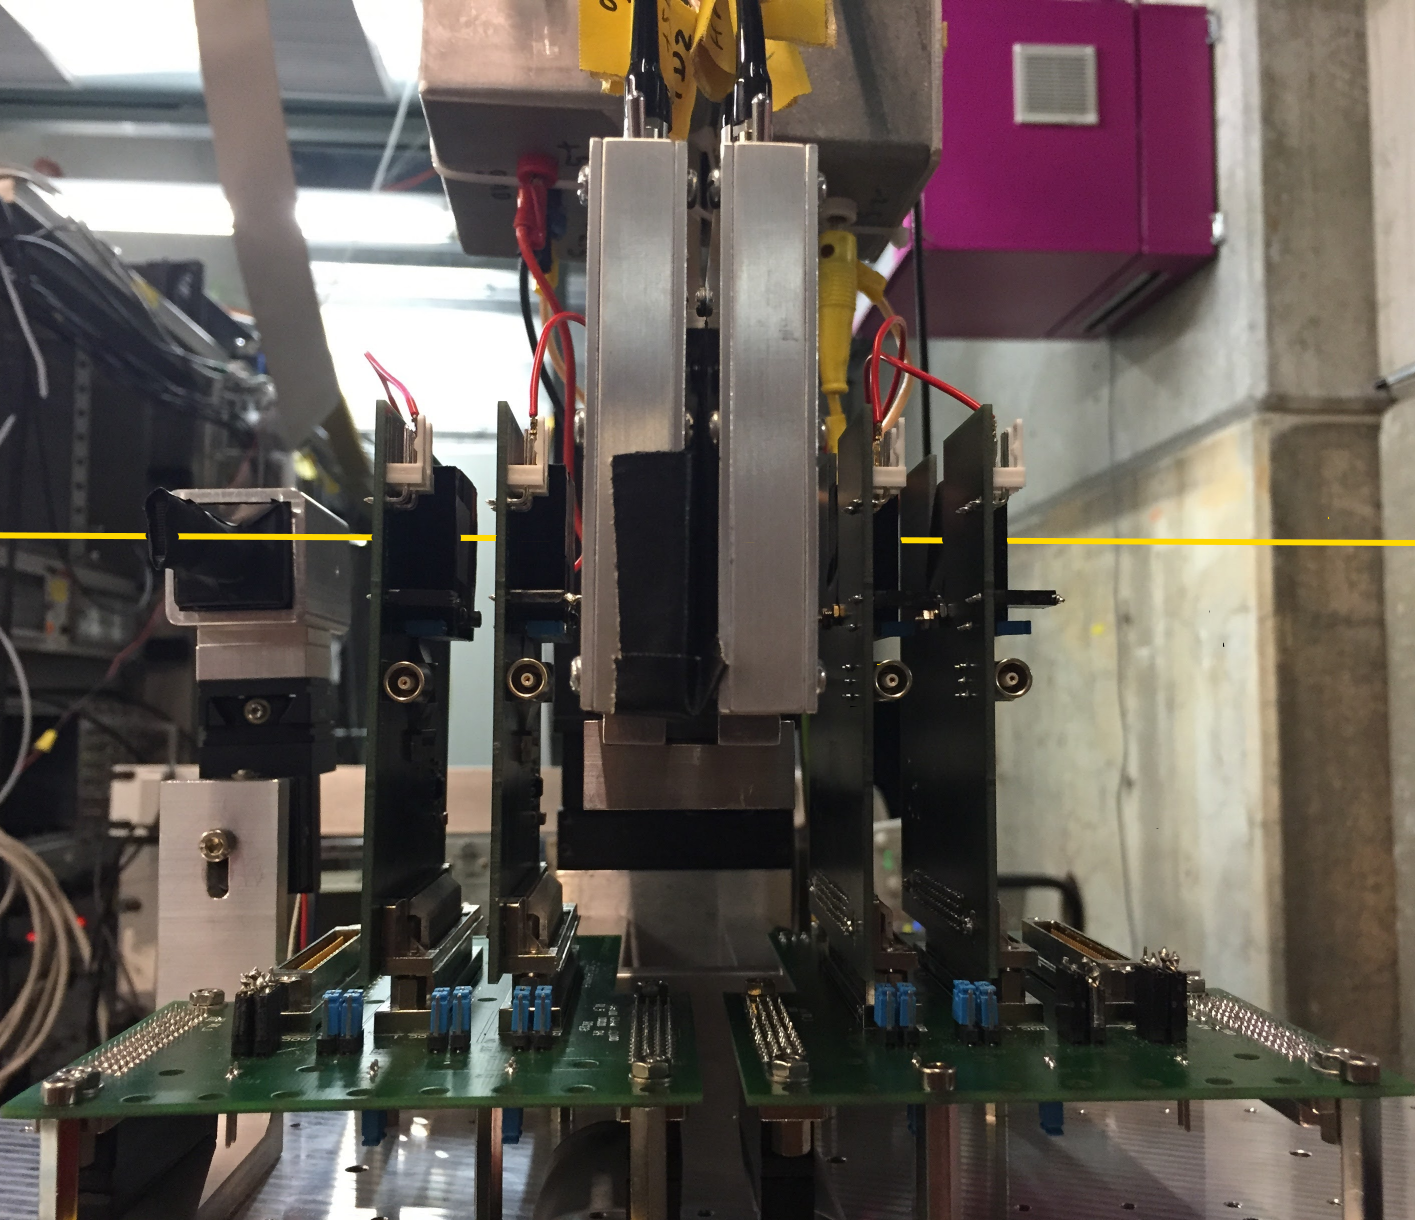
\includegraphics[width=4cm]{telescope3}
	\end{center}
	\begin{alertblock}{
		\begin{center}
			\textbf{Rate Pad Analysis Summary (I)}
		\end{center}}
		\vspace*{10pt}
		\begin{center}\small
		Michael Reichmann
		\end{center}\normalsize
	\end{alertblock}
\end{frame}
% END
% ============================
% BEGIN TABLE OF CONTENTS
% ============================
\begin{frame}[allowframebreaks]
	\frametitle{Table of contents}
	\tableofcontents %[pausesections]
\end{frame}
% END
% ====================================================================================
% BEGIN INTRO
% ====================================================================================
\section{Introduction}
% ====================================================================================
\subsection{Applicability}
\begin{frame}
	\begin{itemize}
		\setlength{\itemsep}{\fill}
		\item analysis fully applicable for all pad runs of the PSI August and October 2015 beam test data
		\item tested diamonds
		\begin{itemize}
			\item August: II6-97, II6-B2, S129, poly-B
			\item October: II6-97, II6-B2, S129, poly-D, 2A87-E, IIa-3
		\end{itemize}
		\item examples during this presentation either show S129 or II6-B2 of the October beam test data
		\item need to extend analysis to PSI May 2015 beam test data
		\begin{itemize}
			\item same dataformat
			\item less precise timing (no scintillator)
			\item different run logging
		\end{itemize}
	\end{itemize}
\end{frame}
% ====================================================================================
\subsection{Setup}
\begin{frame}
	\begin{center}
		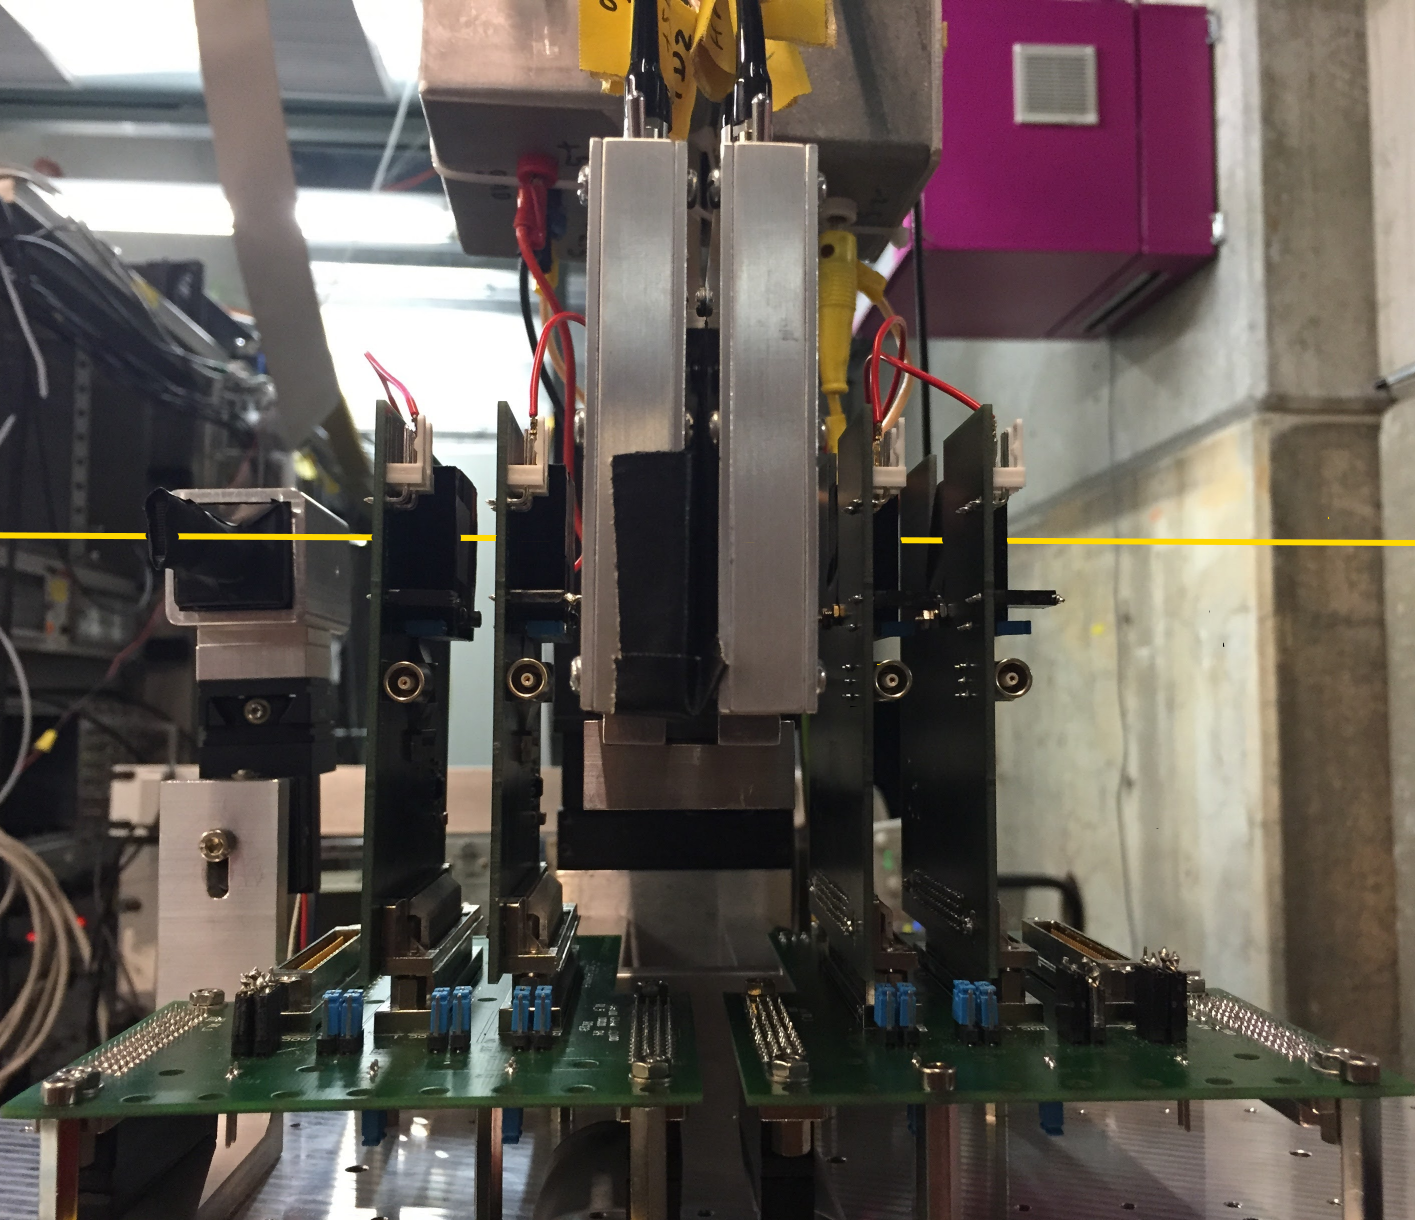
\includegraphics[width=6cm]{telescope3}
	\end{center}
	\begin{itemize}
		\item four analogue CMS Pixel planes connected to a Digtial Test Board (DTB)
		\item two diamond pad detectors connected to a DRS4 Evaluation Board
		\item a scinitallator for precise timing
	\end{itemize}
\end{frame}
% ====================================================================================
\subsection{Datataking}
\begin{frame}
	\begin{center}
		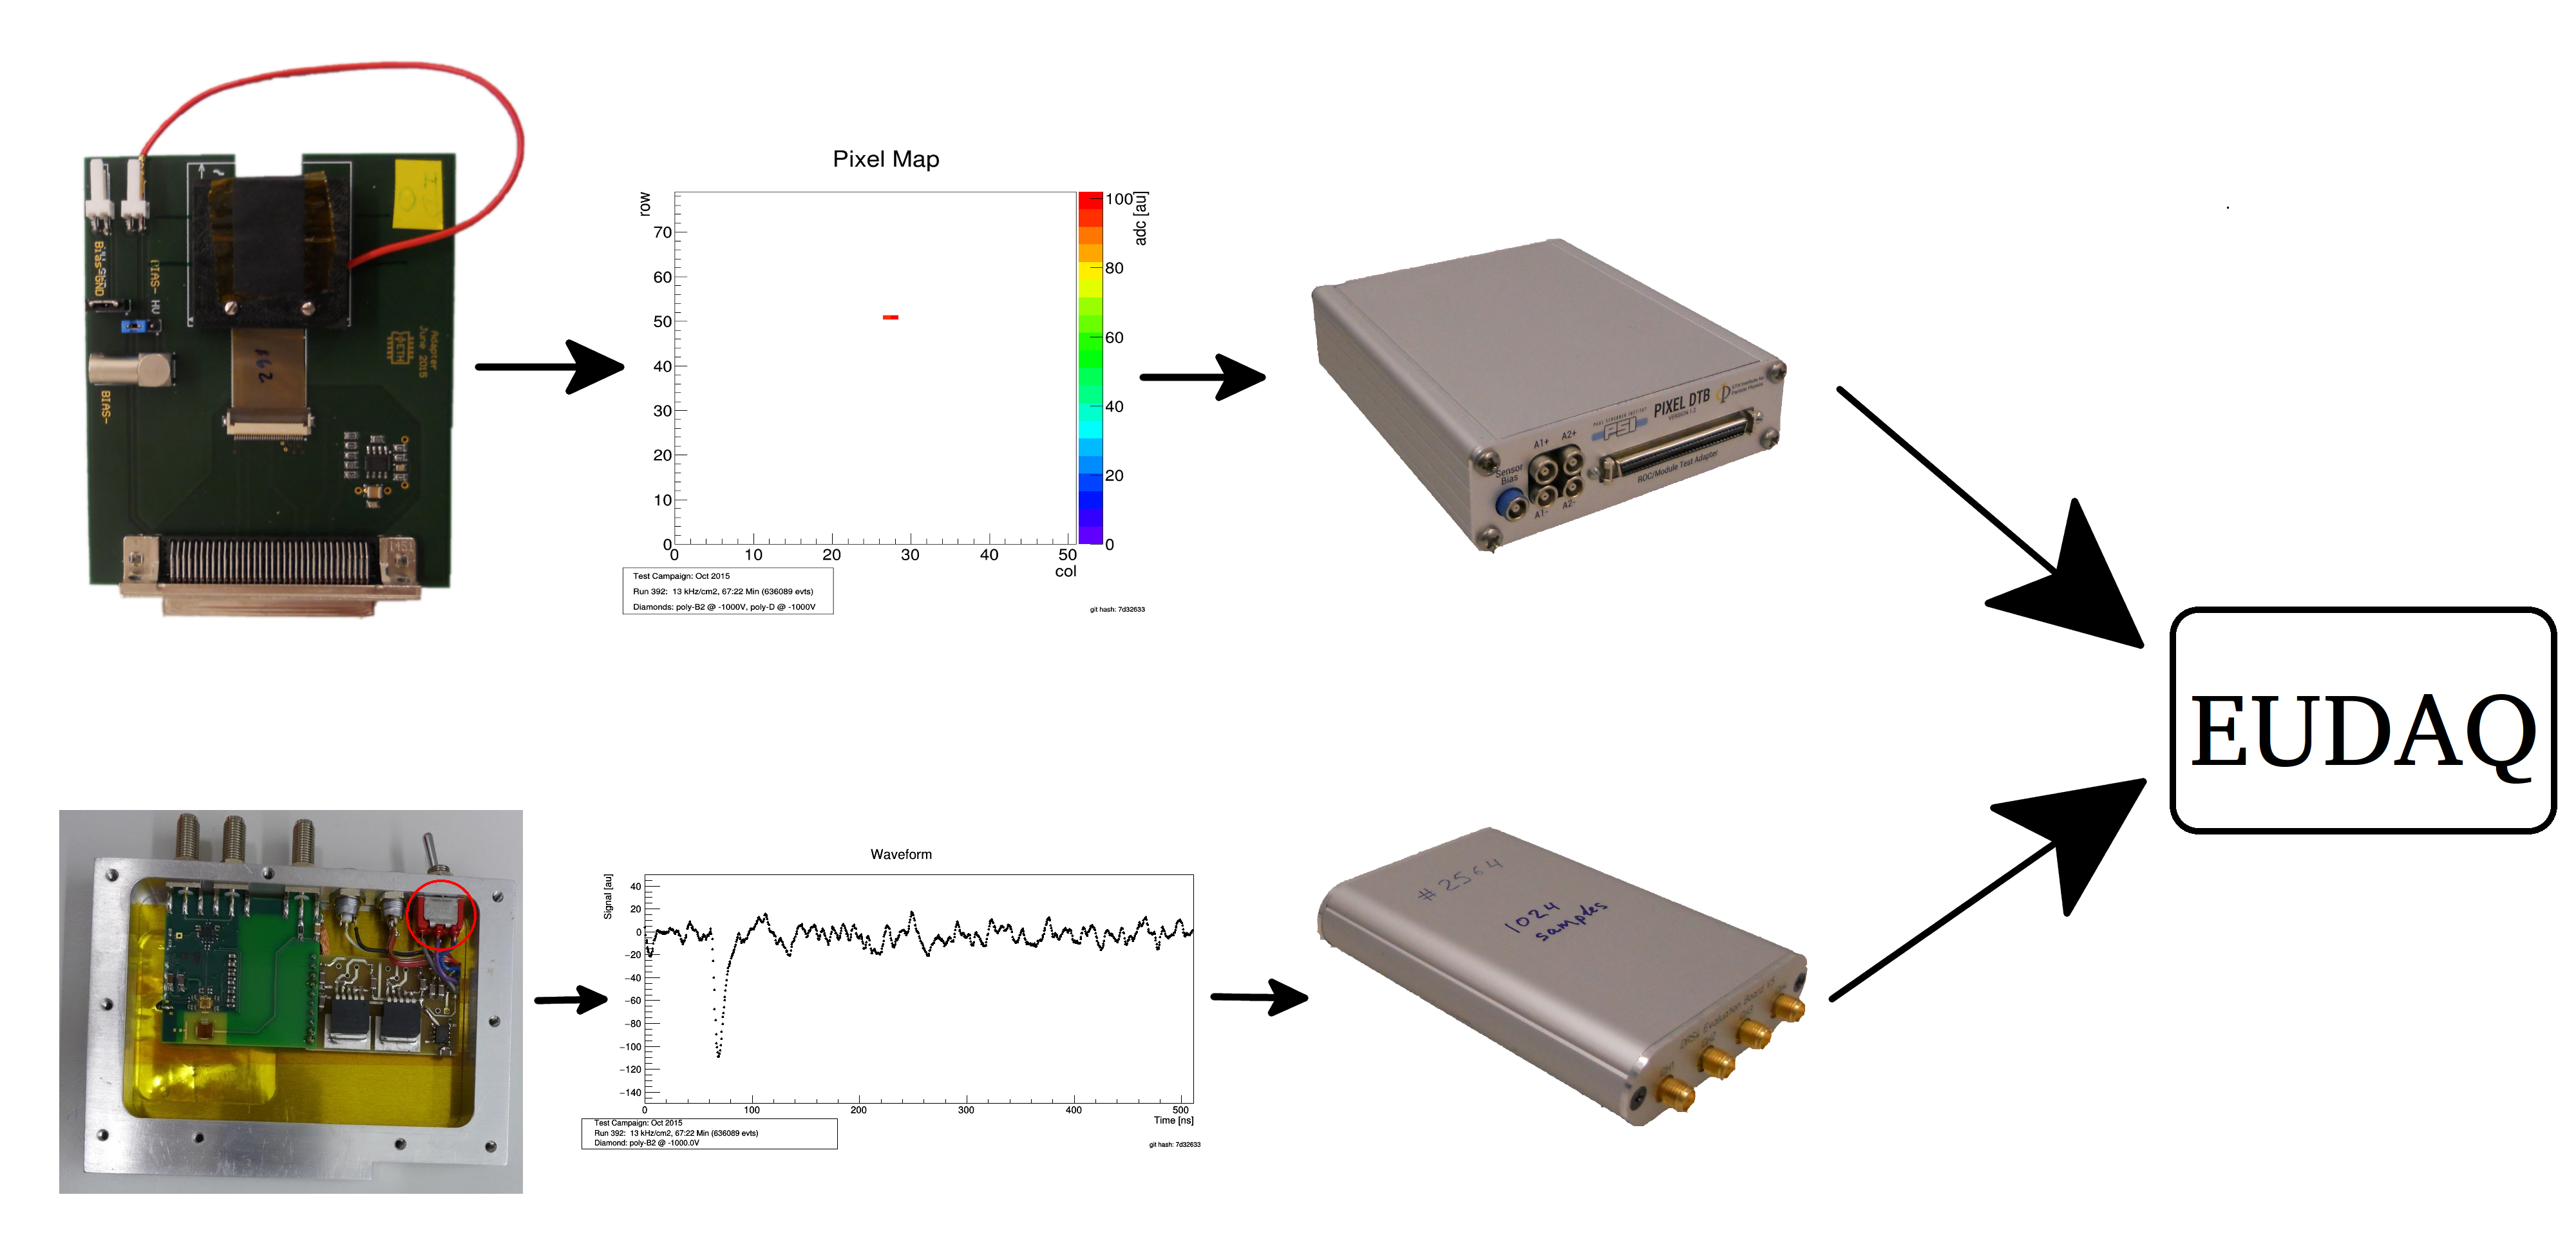
\includegraphics[width=\textwidth]{Intro}
	\end{center}
	\begin{itemize}
		\item EUDAQ saves event based data stream as binary file
		\item require conversion to readable data (i.e. ROOT)
	\end{itemize}
\end{frame}
% END INTRO
% ====================================================================================
% BEGIN CONVERTER
% ====================================================================================
\section{EUDAQ Converter}
\begin{frame}
	\begin{itemize}
		\setlength{\itemsep}{\fill}
		\item EUDAQ already has a converter for binary files (e.g. for CMS Pixel events)
		\item had no converter for drs4 events
		\item wrote our own drs4tree converter based on the existing stuff by Felix (various iterations)
		\item goals of the converter:
		\begin{itemize}
			\item conversion of the binary data into an (event based) root tree
			\item extraction of pulse height information of the Signal, Pedestal and Pulser
		\end{itemize}
		\item idea for signal extraction:
		\begin{itemize}
			\item look for the maximum amplitude of the waveform within a predefined interval
			\begin{itemize}
				\item \textcolor{red}{\textbf{PeakSearchRegion}} (short: Region)
			\end{itemize}
			\item integration of the waveform around this maximum value within another given interval: 
			\begin{itemize}
				\item \textcolor{red}{\textbf{IntegralRange}}
			\end{itemize}
		\end{itemize}
	\item define a user-defined number of \textbf{PeakSearchRegion} and \textbf{IntegralRanges} in a configuration file
	\end{itemize}
\end{frame}
% ====================================================================================
\subsection{Definition of the PeakSearchRegions}
\begin{frame}
\frametitle{Regions}
\begin{itemize}
	\setlength{\itemsep}{\fill}
	\item define \textbf{PeakSearchRegion} (and \textbf{IntegralRanges}) for every stable setup (i.e. same trigger logic) during a beam test
	\item \textbf{Regions} found by visual inspections of some raw waveforms
	\begin{itemize}
		\item waveforms extracted by small script that grabs n waveforms from a single run (preferrably low rate)
		\item waveforms already have the pulser flag
		\item proven that the position of the waveform is very stable for the same setup
	\end{itemize}
	\item Pedestal Region:
	\begin{itemize}
		\item chosen relative to the most probable Signal Peak Position
		\item put at the position one particle bunch (bucket) (\SI{20}{ns} or \SI{40}{DRS4 Units}) before the triggered signal peak (almost no signals there)
		\item thus fixed position for the integration (still called Region)
		\item reason: catch the full signal if there is still one (and be able to cut for it)
	\end{itemize}
	\item may define other regions as reference
\end{itemize}
\end{frame}
% ====================================================================================
\subsection{Waveforms}
\begin{frame}
	\frametitle{Signal}
	\begin{center}
		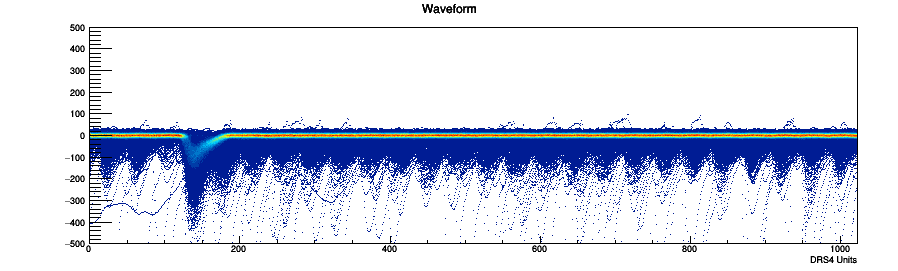
\includegraphics[width=10cm]{WF0}\\
		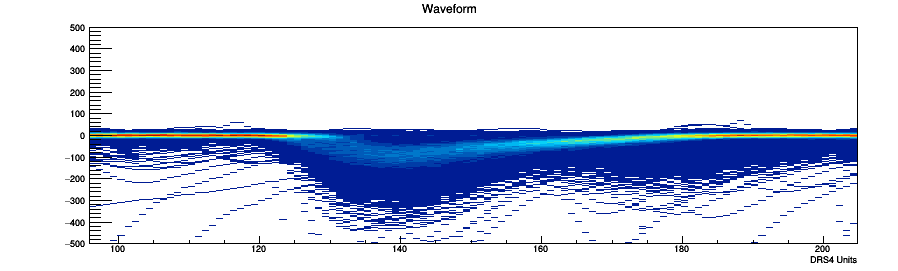
\includegraphics[width=10cm]{WF1}\\
	\end{center}
	\begin{itemize}
		\item Signal Region: $[120,160]$
	\end{itemize}
\end{frame}
% new frame ============================
\begin{frame}
	\begin{center}
		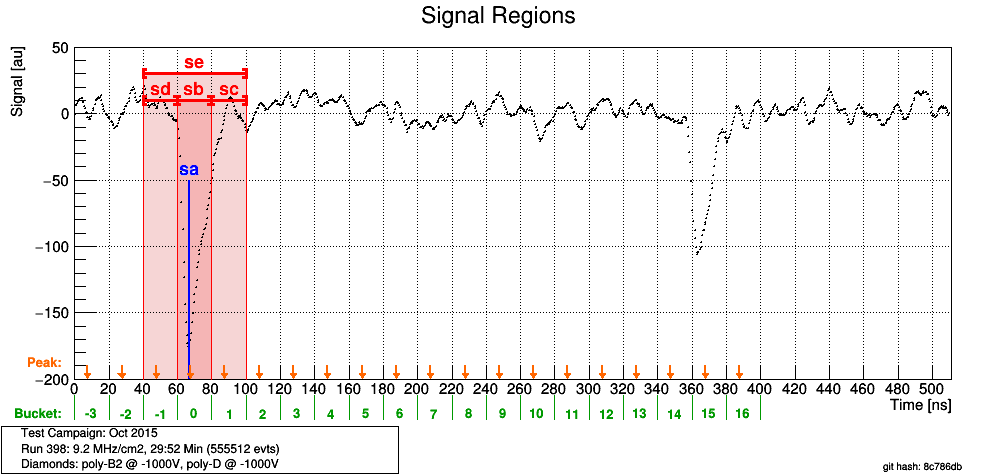
\includegraphics[width=10cm]{SignalRegions}
	\end{center}
	\begin{itemize}
		\item final choice of the regions
		\item explanation later
	\end{itemize}
\end{frame}
% new frame ============================
\begin{frame}
	\frametitle{Pulser}
	\begin{center}
		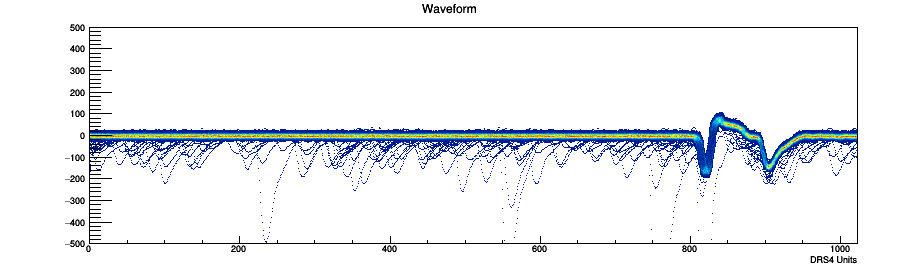
\includegraphics[width=10cm]{WF2}\\
		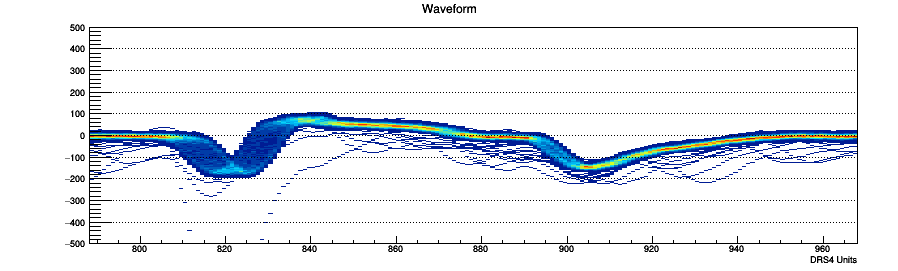
\includegraphics[width=10cm]{WF3}\\
	\end{center}
	\begin{itemize}
		\item Pulser Region: $[880,940]$
	\end{itemize}
\end{frame}
% new frame ============================
\begin{frame}
	\frametitle{Pedestal}
	\begin{center}
		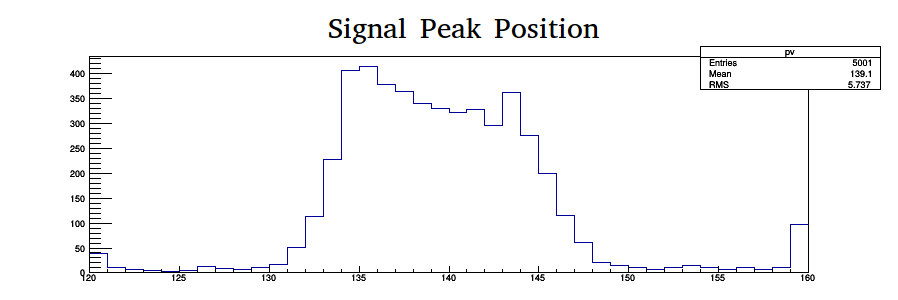
\includegraphics[width=10cm]{PeakValues}
	\end{center}
	\begin{itemize}
		\item MPV at \SI{135}{DRS4 Units}
		\item Pedestal Region: $[95,96]$
	\end{itemize}
\end{frame}
% ====================================================================================
\subsection{Definition of the Integral Ranges}
\begin{frame}
	\frametitle{IntegralRange}
	\begin{center}
		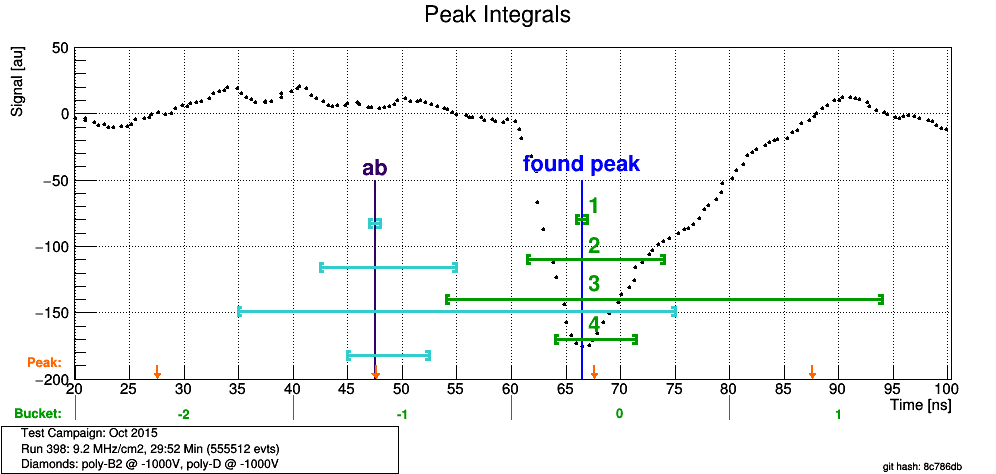
\includegraphics[width=9cm]{IntegralPeaks}
	\end{center}
	\begin{itemize}
		\item applied for every PeakSearchRegions
		\item great influence on the Signal to Noise Ratio (SNR) (ratio of signal integral over sigma of the pedestal)
		\item strongly dependend on the shape of the waveform
		\item best setting found with SNR optimisation $\rightarrow$ Analysis Part
		\begin{itemize}
			\item $[8,12]$: Integration from \SI{8}{DRS4 Units} before and \SI{12}{DRS4 Units} after the found peak
		\end{itemize}

	\end{itemize}
\end{frame}
% END CONVERTER
% ====================================================================================
% TELESCOPE ANALYSIS
% ====================================================================================
\section{Telescope Analysis}
\subsection{Tracks}
\begin{frame}
\end{frame}
% ====================================================================================
\subsection{\texorpdfstring{$\upchi^{2}$}{chi2}}
\begin{frame}
\end{frame}
% ====================================================================================
\subsection{Track Angle}
\begin{frame}
\end{frame}
% ====================================================================================
% CUTS
% ====================================================================================
\section{Cuts}
\subsection{Tracks}
\begin{frame}
\end{frame}
% ====================================================================================
\subsection{Signal}
\begin{frame}
\end{frame}
% ====================================================================================
% WF ANALYSIS
% ====================================================================================
\section{Analysis I (Waveforms)}
% ====================================================================================
\subsection{Pedestal}
\begin{frame}
\end{frame}
% ====================================================================================
\subsection{Signal}
\begin{frame}
\end{frame}
% ====================================================================================
\subsection{Pulser}
\begin{frame}
\end{frame}
% ====================================================================================
% WF ANALYSIS
% ====================================================================================
\section{Analysis II}
% ====================================================================================
% ====================================================================================
\subsection{Beam Profile}
\begin{frame}
\end{frame}
% ====================================================================================
\subsection{Signal Peak Positions in Time}
\begin{frame}
\end{frame}
% ====================================================================================
\subsection{2D Signal Maps}
\begin{frame}
\end{frame}
% ====================================================================================
\subsection{Diamond Currents}
\begin{frame}
\end{frame}

% ============================
% DOCUMENT END
\end{document}

